% Бүлэг 4

\chapter{Платформын архитектур ба системийн бүтэц}
\label{Chapter4}

\section{Бүлгийн зорилго}
Энэ бүлэгт өмнөх бүлэгт тайлбарласан хэрэгжилтийг системийн архитектурын түвшинд нэгтгэн авч үзнэ. Гуравдугаар бүлэг нь \textit{ямар модулийг хэрхэн хэрэгжүүлсэн бэ?} гэдэгт төвлөрсөн бол дөрөвдүгээр бүлэг нь \textit{эдгээр модуль хоорондоо хэрхэн холбогдож, ямар давхарга, ямар өгөгдлийн урсгал, ямар бүтцээр систем болж ажиллаж байна вэ?} гэдэгт хариулна.

Архитектурын судалгаанд дараах асуудлыг хамруулав.
\begin{itemize}
  \item системийн логик давхарга ба хариуцлагын зааг;
  \item хэрэглэгч, админ, AI provider, Supabase зэрэг гаднын оролцогчийн холбоо;
  \item use case, activity, sequence, class, ER диаграмын тайлбар;
  \item frontend, application, API, data, AI support, dataset давхаргын бүтэц;
  \item security, scalability, maintainability, deployment-ийн архитектурын шийдэл;
  \item ирээдүйн өргөтгөлийн архитектурын чиглэл.
\end{itemize}

\section{Системийн ерөнхий архитектур}
FL Studio сургалтын платформ нь сургалтын контент, хэрэглэгчийн эрх, суралцах явц, AI туслах, dataset pipeline гэсэн таван гол бүрэлдэхүүнээс бүрдэнэ. Эдгээрийг нэг кодын бааз дотор бүрэн хольж бичвэл систем засварлахад хүндрэлтэй болно. Иймээс архитектурын үндсэн зарчим нь \textbf{давхарга тусгаарлах}, \textbf{өгөгдлийн ownership тодорхойлох}, \textbf{AI-г туслах давхарга байдлаар хязгаарлах}, \textbf{өргөтгөх боломж хадгалах} юм.

\begin{figure}[htbp]
  \centering
  \resizebox{\textwidth}{!}{\begin{tikzpicture}[x=1cm,y=1cm,>=stealth,thick]
  \tikzstyle{layer}=[draw, rounded corners=5pt, minimum width=13.5cm, minimum height=1.0cm, align=center]
  \tikzstyle{side}=[draw, rounded corners=4pt, minimum width=3.5cm, minimum height=0.8cm, align=center, font=\small]

  \node[layer, fill=blue!8] (ui) at (0,0) {\textbf{Танилцуулгын давхарга}\\Веб хуудас, компонент, хэрэглэгчийн интерфейс, курс/хичээл/чат};
  \node[layer, fill=green!8] (app) at (0,-1.8) {\textbf{Аппликейшний давхарга}\\Клиент төлөвийн функц, хандалтын хяналт, хичээлийн урсгал, сорилын төлөв};
  \node[layer, fill=yellow!10] (api) at (0,-3.6) {\textbf{Хиймэл оюуны туслах давхарга}\\Програмчлалын интерфейсийн зам, сэргээн хайлт, зааварчилгаа, нөөц хариу};
  \node[layer, fill=orange!10] (data) at (0,-5.4) {\textbf{Өгөгдлийн давхарга}\\Үүлэн харилцаат өгөгдлийн сан, нэвтрэлт, мөрийн түвшний хамгаалалт, ахиц};
  \node[layer, fill=gray!14] (assets) at (0,-7.2) {\textbf{Контент ба өгөгдлийн багцын давхарга}\\Курсийн эх өгөгдөл, видео хичээлийн лавлагаа, өгөгдлийн багц, ФЛ Студио зөвлөмж};

  \draw[->] (ui) -- (app);
  \draw[->] (app) -- (api);
  \draw[->] (api) -- (data);
  \draw[->] (data) -- (assets);

  \node[side, fill=purple!8] (student) at (-9.0,-0.9) {Суралцагч};
  \node[side, fill=purple!8] (admin) at (9.0,-0.9) {Админ};
  \node[side, fill=cyan!8] (llm) at (9.0,-3.6) {Хэлний загварын үйлчилгээ};
  \node[side, fill=cyan!8] (supabase) at (9.0,-5.4) {Үүлэн сангийн үйлчилгээ};

  \draw[->] (student) -- (ui.west);
  \draw[->] (admin) -- (ui.east);
  \draw[->] (api.east) -- (llm);
  \draw[->] (data.east) -- (supabase);
\end{tikzpicture}
}
  \caption[Платформын давхаргат архитектур]{Платформын давхаргат архитектур}
  \label{fig:layered-architecture}
\end{figure}

Зураг \ref{fig:layered-architecture}-д системийн үндсэн давхаргыг харуулав. Presentation layer нь хэрэглэгчийн интерфейсийг хариуцна. Application layer нь user flow, access control, lesson state, quiz state, admin workflow зэрэг бизнес логикийг frontend талд зохицуулна. API and AI support layer нь chatbot, YouTube duration, provider abstraction зэрэг server-side logic-ийг агуулна. Data layer нь Supabase PostgreSQL, authentication, RLS, course/progress/payment/knowledge base өгөгдлийг удирдана. Content and Dataset layer нь course seed data, YouTube lesson reference, RAG JSONL/CSV, generated FL Studio tips зэрэг сургалтын болон AI өгөгдлийн эх үүсвэрийг хадгална.

\section{Оролцогч ба use case бүтэц}
Системийн use case нь зочин, суралцагч, админ гэсэн гурван үндсэн actor-той. Зочин хэрэглэгч курс хайх, free preview үзэх, бүртгүүлэх боломжтой. Суралцагч бүртгэлээр нэвтэрч, курс худалдан авч, lesson үзэж, self-check quiz өгч, AI mentor-оос асуулт асууж, ахицаа хадгална. Админ course, lesson, knowledge base, хэрэглэгчийн мэдээллийг удирдана.

\begin{figure}[htbp]
  \centering
  \resizebox{0.95\textwidth}{!}{\definecolor{ucslate}{HTML}{475569}
\definecolor{ucsky}{HTML}{38BDF8}
\definecolor{ucemerald}{HTML}{34D399}
\definecolor{ucamber}{HTML}{FBBF24}
\definecolor{ucindigo}{HTML}{818CF8}

\begin{tikzpicture}[
  x=1cm,
  y=1cm,
  >=stealth,
  font=\sffamily\small,
  actorline/.style={draw=ucslate!70, line width=0.9pt, line cap=round},
  actorlabel/.style={font=\sffamily\small\bfseries, align=center, text=ucslate!80},
  boundary/.style={draw=ucslate!55, line width=1.1pt, rounded corners=16pt, fill=gray!2},
  band/.style={draw=gray!25, line width=0.5pt, rounded corners=10pt},
  usecase/.style={
    draw=ucslate!55,
    line width=0.8pt,
    ellipse,
    align=center,
    minimum width=4.6cm,
    minimum height=1.3cm,
    inner xsep=8pt,
    inner ysep=4pt,
    font=\sffamily\small,
    drop shadow={shadow xshift=0.4pt, shadow yshift=-0.4pt, fill=gray!15, opacity=0.35}
  },
  publiccase/.style={usecase, fill=ucsky!12},
  learncase/.style={usecase, fill=ucemerald!10},
  aicase/.style={usecase, fill=ucamber!12},
  admincase/.style={usecase, fill=ucindigo!8},
  relation/.style={draw=ucslate!45, line width=0.7pt},
  include/.style={draw=ucslate!60, dashed, ->, line width=0.7pt},
  notelabel/.style={font=\sffamily\scriptsize\itshape, fill=white, inner sep=1.5pt, text=ucslate!60}
]

  % ── System boundary ──
  \draw[boundary] (0,0) rectangle (17,11.5);
  \fill[ucslate!10, rounded corners=16pt] (0.02,10.4) rectangle (16.98,11.48);
  \node[font=\sffamily\bfseries, text=ucslate!75] at (8.5,10.94)
    {FL Studio сургалтын AI дэмжлэгтэй веб платформ};

  % ── Zone bands ──
  \draw[band, fill=ucsky!5] (0.5,8.3) rectangle (16.5,10.2);
  \node[font=\sffamily\scriptsize\bfseries, text=ucsky!70!black, anchor=north west]
    at (0.8,10.15) {Нийтийн хэрэглээ};

  \draw[band, fill=ucemerald!5] (0.5,4.5) rectangle (16.5,8.0);
  \node[font=\sffamily\scriptsize\bfseries, text=ucemerald!60!black, anchor=north west]
    at (0.8,7.95) {Суралцах урсгал};

  \draw[band, fill=ucamber!6] (0.5,0.5) rectangle (16.5,4.2);
  \node[font=\sffamily\scriptsize\bfseries, text=ucamber!70!black, anchor=north west]
    at (0.8,4.15) {AI туслах ба админ удирдлага};

  % ── Use cases: Public ──
  \node[publiccase] (auth)    at (3.8,9.2) {Бүртгүүлэх, Нэвтрэх};
  \node[publiccase] (browse)  at (8.5,9.2) {Курс хайх, шүүх};
  \node[publiccase] (preview) at (13.2,9.2) {Үнэгүй танилцах\\хичээл үзэх};

  % ── Use cases: Learning ──
  \node[learncase] (purchase) at (3.8,6.8)  {Курс худалдан авах};
  \node[learncase] (lesson)   at (8.5,6.8)  {Хичээл үзэх};
  \node[learncase] (quiz)     at (13.2,6.8) {Өөрийгөө шалгах\\сорил өгөх};
  \node[learncase] (progress) at (13.2,5.3) {Явц хадгалах};

  % ── Use cases: AI & Admin ──
  \node[aicase] (chat)   at (3.8,2.8)  {AI туслахаас асуух};
  \node[aicase] (source) at (8.5,2.8)  {Эх сурвалжтай\\хариу авах};
  \node[admincase] (adminContent)   at (13.2,3.3) {Курс ба хичээл\\удирдах};
  \node[admincase] (adminKnowledge) at (13.2,1.7) {Мэдлэгийн сан\\удирдах};

  % ── Guest actor ──
  \node[draw=ucsky!60!black, circle, fill=ucsky!12, minimum size=0.7cm, line width=0.8pt] at (-1.8,9.3) {};
  \draw[actorline] (-1.8,8.95) -- (-1.8,8.05);
  \draw[actorline] (-2.25,8.55) -- (-1.35,8.55);
  \draw[actorline] (-1.8,8.05) -- (-2.2,7.4);
  \draw[actorline] (-1.8,8.05) -- (-1.4,7.4);
  \node[actorlabel] at (-1.8,7.0) {Зочин};
  \coordinate (guest) at (-1.2,8.55);

  % ── Student actor ──
  \node[draw=ucemerald!55!black, circle, fill=ucemerald!10, minimum size=0.7cm, line width=0.8pt] at (-1.8,5.5) {};
  \draw[actorline] (-1.8,5.15) -- (-1.8,4.25);
  \draw[actorline] (-2.25,4.75) -- (-1.35,4.75);
  \draw[actorline] (-1.8,4.25) -- (-2.2,3.6);
  \draw[actorline] (-1.8,4.25) -- (-1.4,3.6);
  \node[actorlabel] at (-1.8,3.2) {Суралцагч};
  \coordinate (student) at (-1.2,4.75);

  % ── Admin actor ──
  \node[draw=ucindigo!60!black, circle, fill=ucindigo!10, minimum size=0.7cm, line width=0.8pt] at (18.8,3.3) {};
  \draw[actorline] (18.8,2.95) -- (18.8,2.05);
  \draw[actorline] (18.35,2.55) -- (19.25,2.55);
  \draw[actorline] (18.8,2.05) -- (18.4,1.4);
  \draw[actorline] (18.8,2.05) -- (19.2,1.4);
  \node[actorlabel] at (18.8,1.0) {Админ};
  \coordinate (admin) at (18.25,2.55);

  % ── Actor connections ──
  \draw[relation] (guest) -- (auth.west);
  \draw[relation] (guest) -- (browse.west);
  \draw[relation] (guest) -- (preview.west);

  \draw[relation] (student) -- (auth.west);
  \draw[relation] (student) -- (purchase.west);
  \draw[relation] (student) -- (lesson.west);
  \draw[relation] (student) -- (quiz.west);
  \draw[relation] (student) -- (progress.west);
  \draw[relation] (student) -- (chat.west);

  \draw[relation] (admin) -- (adminContent.east);
  \draw[relation] (admin) -- (adminKnowledge.east);

  % ── Stereotype relationships ──
  \draw[include] (preview) -- (auth);
  \node[notelabel] at (8.5,9.8) {$\ll$extend$\gg$};

  \draw[include] (purchase) -- (lesson);
  \node[notelabel] at (6.15,7.15) {$\ll$include$\gg$};

  \draw[include] (lesson) -- (quiz);
  \node[notelabel] at (10.85,7.15) {$\ll$include$\gg$};

  \draw[include] (quiz) -- (progress);
  \node[notelabel] at (14.3,6.1) {$\ll$include$\gg$};

  \draw[include] (chat) -- (source);
  \node[notelabel] at (6.15,3.15) {$\ll$include$\gg$};
\end{tikzpicture}
}
  \caption[Use Case диаграм]{FL Studio сургалтын платформын Use Case диаграм}
  \label{fig:ch4-usecase}
\end{figure}

\begin{longtable}{|p{0.18\textwidth}|p{0.24\textwidth}|p{0.42\textwidth}|}
  \caption{Use case тайлбар}
  \label{tab:usecase-description}\\
  \hline
  \textbf{Actor} & \textbf{Use case} & \textbf{Тайлбар} \\ \hline
  Зочин & Курс хайх/шүүх & Системд бүртгүүлээгүй хэрэглэгч course catalog-оос өөрт тохирох сургалтын чиглэл хайна. \\ \hline
  Зочин & Free preview үзэх & Бүртгэл хийхээс өмнө course-ийн эхний lesson, танилцуулга, сургалтын чиглэлийг шалгаж үзнэ. \\ \hline
  Зочин & Бүртгүүлэх/нэвтрэх & Free preview-ээс цааш ахиц хадгалах, төлбөртэй lesson авахын тулд account үүсгэнэ. \\ \hline
  Суралцагч & Хичээл үзэх & Free lesson эсвэл purchased course-ийн lesson үзнэ. \\ \hline
  Суралцагч & Self-check quiz өгөх & Lesson ойлголтоо шалгаж, course progress-д утга нэмнэ. \\ \hline
  Суралцагч & Явц хадгалах & Үзсэн lesson, бөглөсөн quiz, course completion зэрэг суралцах төлөвийг бүртгэнэ. \\ \hline
  Суралцагч & Chatbot-оос асуух & FL Studio, mixing, mastering, music theory-ийн асуултад context-aware зөвлөгөө авна. \\ \hline
  Суралцагч & Эх сурвалжтай хариу авах & AI mentor нь RAG мэдлэгийн сангаас авсан context, source metadata-д тулгуурлан хариулт үүсгэнэ. \\ \hline
  Суралцагч & Курс худалдан авах & Paid content access нээх business flow. \\ \hline
  Админ & Course/Lesson удирдах & Контентын бүтэц, үнэ, ангилал, lesson metadata-г засварлана. \\ \hline
  Админ & Knowledge base удирдах & RAG chatbot-ийн эх сурвалж, асуулт-хариулт, category-г хянаж сайжруулна. \\ \hline
\end{longtable}

\section{Үйл ажиллагааны урсгал}
Суралцагчийн үндсэн workflow нь course discovery-оос эхэлж, access check, lesson, quiz, chatbot, progress хадгалалт гэсэн дараалалтай. Энэ урсгалд chatbot нь үндсэн сургалтыг тасалдуулахгүйгээр туслах функц хэлбэрээр байрлана.

\begin{figure}[htbp]
  \centering
  \resizebox{0.80\textwidth}{!}{\begin{tikzpicture}[
  x=1cm,
  y=1cm,
  >=stealth,
  font=\sffamily\small,
  flow/.style={->, draw=blue!45!black, line width=0.8pt},
  activity/.style={
    draw=blue!55!black,
    fill=blue!4,
    rounded corners=6pt,
    minimum width=4.35cm,
    minimum height=0.86cm,
    align=center,
    line width=0.75pt
  },
  decision/.style={
    diamond,
    draw=orange!60!black,
    fill=orange!8,
    aspect=2.45,
    minimum width=3.85cm,
    minimum height=1.12cm,
    align=center,
    inner xsep=1pt,
    line width=0.75pt
  },
  terminal/.style={circle, draw=blue!55!black, fill=blue!70!black, minimum size=0.50cm, inner sep=0pt},
  flowlabel/.style={font=\sffamily\scriptsize, fill=white, inner sep=1.2pt, text=gray!35!black}
]
  \node[terminal] (start) at (0,0) {};
  \node[activity] (login) at (0,-1.05) {Нэвтрэх / бүртгүүлэх};
  \node[activity] (catalog) at (0,-2.25) {Курсийн каталог үзэх};
  \node[activity] (course) at (0,-3.45) {Курс сонгох};
  \node[decision] (access) at (0,-4.90) {Үзэх эрхтэй\\юу?};
  \node[activity] (buy) at (-4.75,-6.10) {Курс худалдан авах};
  \node[activity] (lesson) at (0,-7.20) {Хичээл үзэх};
  \node[activity] (quiz) at (0,-8.45) {Өөрийгөө шалгах};
  \node[decision] (help) at (0,-9.90) {Тусламж\\хэрэгтэй юу?};
  \node[activity] (chat) at (4.75,-11.10) {AI туслахаас асуух};
  \node[activity] (progress) at (0,-12.30) {Ахиц хадгалах};
  \node[terminal] (end) at (0,-13.40) {};

  \draw[flow] (start) -- (login);
  \draw[flow] (login) -- (catalog);
  \draw[flow] (catalog) -- (course);
  \draw[flow] (course) -- (access);
  \draw[flow] (access.west) -- node[flowlabel, above] {Үгүй} (buy.east);
  \draw[flow] (buy.south) |- (lesson.west);
  \draw[flow] (access.south) -- node[flowlabel, right] {Тийм} (lesson.north);
  \draw[flow] (lesson) -- (quiz);
  \draw[flow] (quiz) -- (help);
  \draw[flow] (help.east) -- node[flowlabel, above] {Тийм} (chat.west);
  \draw[flow] (chat.south) |- (progress.east);
  \draw[flow] (help.south) -- node[flowlabel, left] {Үгүй} (progress.north);
  \draw[flow] (progress) -- (end);
\end{tikzpicture}
}
  \caption[Суралцагчийн үйл ажиллагааны диаграм]{Суралцагчийн үйл ажиллагааны диаграм}
  \label{fig:ch4-activity}
\end{figure}

Activity diagram-аас харахад төлбөртэй access нь lesson flow-ийн өмнөх шийдвэрийн цэг юм. Хэрэв access байхгүй бол хэрэглэгч purchase flow руу шилжинэ. Access нээгдсэний дараа lesson үзэх, self-check хийх, шаардлагатай үед AI туслахаас асуух, эцэст нь progress хадгалах шат хийгдэнэ.

\section{Класс ба домайн бүтэц}
Системийн домайн объектуудыг User, Course, Lesson, CourseProgress, ChatMessage, Payment зэрэг үндсэн class-аар дүрсэлж болно. Энэ class diagram нь frontend type model, Supabase schema, UI flow гурвыг нэгтгэн ойлгоход тусална.

\begin{figure}[htbp]
  \centering
  \resizebox{\textwidth}{!}{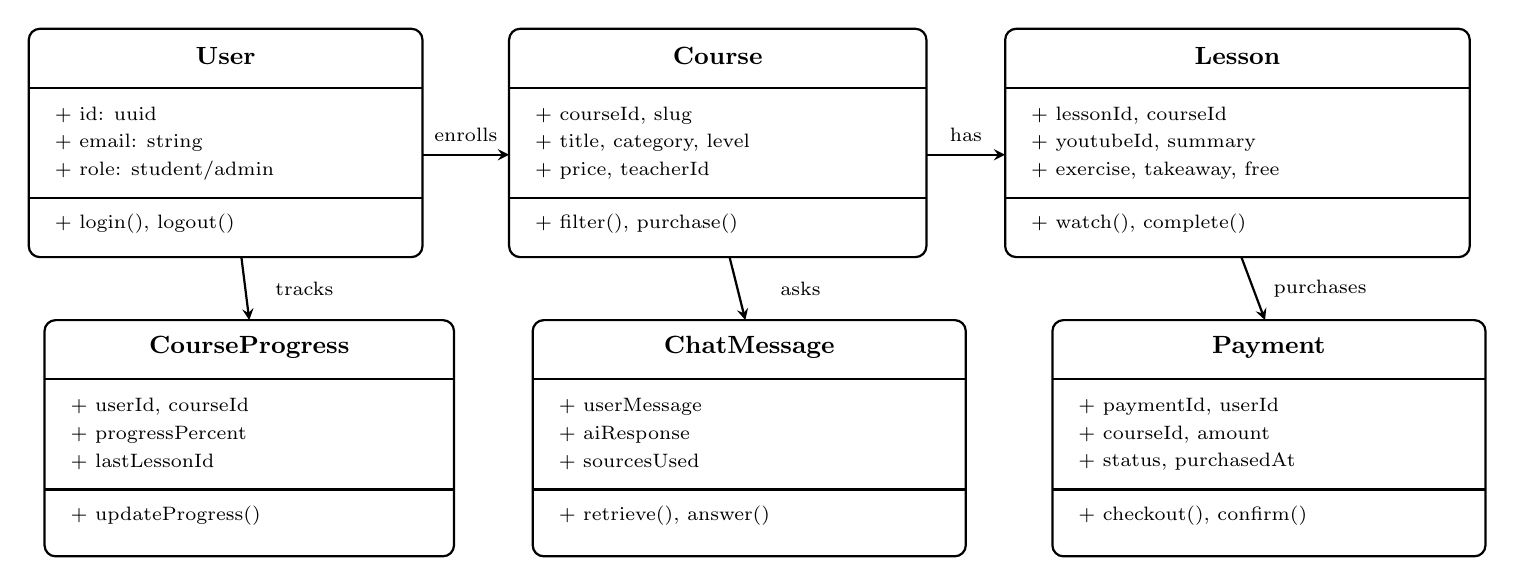
\begin{tikzpicture}[x=1cm,y=1cm,>=stealth,thick]
  \draw[rounded corners=4pt] (0,6.3) rectangle (5.0,9.2);
  \node[font=\small\bfseries] at (2.5,8.85) {User};
  \draw (0,8.45) -- (5.0,8.45);
  \node[anchor=west,font=\scriptsize] at (0.2,8.1) {+ id: uuid};
  \node[anchor=west,font=\scriptsize] at (0.2,7.75) {+ email: string};
  \node[anchor=west,font=\scriptsize] at (0.2,7.4) {+ role: student/admin};
  \draw (0,7.05) -- (5.0,7.05);
  \node[anchor=west,font=\scriptsize] at (0.2,6.72) {+ login(), logout()};

  \draw[rounded corners=4pt] (6.1,6.3) rectangle (11.4,9.2);
  \node[font=\small\bfseries] at (8.75,8.85) {Course};
  \draw (6.1,8.45) -- (11.4,8.45);
  \node[anchor=west,font=\scriptsize] at (6.3,8.1) {+ courseId, slug};
  \node[anchor=west,font=\scriptsize] at (6.3,7.75) {+ title, category, level};
  \node[anchor=west,font=\scriptsize] at (6.3,7.4) {+ price, teacherId};
  \draw (6.1,7.05) -- (11.4,7.05);
  \node[anchor=west,font=\scriptsize] at (6.3,6.72) {+ filter(), purchase()};

  \draw[rounded corners=4pt] (12.4,6.3) rectangle (18.3,9.2);
  \node[font=\small\bfseries] at (15.35,8.85) {Lesson};
  \draw (12.4,8.45) -- (18.3,8.45);
  \node[anchor=west,font=\scriptsize] at (12.6,8.1) {+ lessonId, courseId};
  \node[anchor=west,font=\scriptsize] at (12.6,7.75) {+ youtubeId, summary};
  \node[anchor=west,font=\scriptsize] at (12.6,7.4) {+ exercise, takeaway, free};
  \draw (12.4,7.05) -- (18.3,7.05);
  \node[anchor=west,font=\scriptsize] at (12.6,6.72) {+ watch(), complete()};

  \draw[rounded corners=4pt] (0.2,2.5) rectangle (5.4,5.5);
  \node[font=\small\bfseries] at (2.8,5.15) {CourseProgress};
  \draw (0.2,4.75) -- (5.4,4.75);
  \node[anchor=west,font=\scriptsize] at (0.4,4.4) {+ userId, courseId};
  \node[anchor=west,font=\scriptsize] at (0.4,4.05) {+ progressPercent};
  \node[anchor=west,font=\scriptsize] at (0.4,3.7) {+ lastLessonId};
  \draw (0.2,3.35) -- (5.4,3.35);
  \node[anchor=west,font=\scriptsize] at (0.4,3.02) {+ updateProgress()};

  \draw[rounded corners=4pt] (6.4,2.5) rectangle (11.9,5.5);
  \node[font=\small\bfseries] at (9.15,5.15) {ChatMessage};
  \draw (6.4,4.75) -- (11.9,4.75);
  \node[anchor=west,font=\scriptsize] at (6.6,4.4) {+ userMessage};
  \node[anchor=west,font=\scriptsize] at (6.6,4.05) {+ aiResponse};
  \node[anchor=west,font=\scriptsize] at (6.6,3.7) {+ sourcesUsed};
  \draw (6.4,3.35) -- (11.9,3.35);
  \node[anchor=west,font=\scriptsize] at (6.6,3.02) {+ retrieve(), answer()};

  \draw[rounded corners=4pt] (13.0,2.5) rectangle (18.5,5.5);
  \node[font=\small\bfseries] at (15.75,5.15) {Payment};
  \draw (13.0,4.75) -- (18.5,4.75);
  \node[anchor=west,font=\scriptsize] at (13.2,4.4) {+ paymentId, userId};
  \node[anchor=west,font=\scriptsize] at (13.2,4.05) {+ courseId, amount};
  \node[anchor=west,font=\scriptsize] at (13.2,3.7) {+ status, purchasedAt};
  \draw (13.0,3.35) -- (18.5,3.35);
  \node[anchor=west,font=\scriptsize] at (13.2,3.02) {+ checkout(), confirm()};

  \draw[->] (5.0,7.6) -- (6.1,7.6);
  \node[font=\scriptsize, fill=white, inner sep=1pt] at (5.55,7.85) {enrolls};
  \draw[->] (11.4,7.6) -- (12.4,7.6);
  \node[font=\scriptsize, fill=white, inner sep=1pt] at (11.9,7.85) {has};
  \draw[->] (2.7,6.3) -- (2.8,5.5);
  \node[font=\scriptsize, fill=white, inner sep=1pt] at (3.5,5.9) {tracks};
  \draw[->] (8.9,6.3) -- (9.1,5.5);
  \node[font=\scriptsize, fill=white, inner sep=1pt] at (9.8,5.9) {asks};
  \draw[->] (15.4,6.3) -- (15.7,5.5);
  \node[font=\scriptsize, fill=white, inner sep=1pt] at (16.4,5.9) {purchases};
\end{tikzpicture}
}
  \caption[Класс диаграм]{Платформын домайн объектуудын класс диаграм}
  \label{fig:ch4-class}
\end{figure}

Class diagram-д Course нь олон Lesson агуулна. User нь Course-д enroll хийх, purchase хийх, progress хадгалах, chat message үүсгэх боломжтой. ChatMessage нь RAG retrieval болон AI response-тэй холбоотой. Payment нь course access-ийн business object болно. Энэ бүтэц нь системийн object model-ийг өгөгдлийн сангийн relational model-тэй холбох суурь болдог.

\section{Өгөгдлийн сангийн архитектур}
\subsection{ER загвар}
Өгөгдлийн сангийн ER загвар нь хэрэглэгчийн бүртгэл, сургалтын контент, худалдан авалт ба ахиц, мөн мэдлэгийн сан ба чат гэсэн дөрвөн бүлэг entity-г нэгтгэнэ.

\begin{figure}[htbp]
  \centering
  \resizebox{\textwidth}{!}{\begin{tikzpicture}[x=1cm,y=1cm,>=stealth,thick]
  \tikzstyle{entity}=[draw, rounded corners=4pt, minimum width=4.6cm, minimum height=2.1cm, align=left, font=\scriptsize]

  \node[entity] (profiles) at (0,6.6) {\textbf{Профайл}\\Үндсэн түлхүүр\\бүтэн нэр\\админ эсэх};
  \node[entity] (courses) at (6.0,6.6) {\textbf{Курс}\\Үндсэн түлхүүр\\курсийн дугаар, товч нэр\\гарчиг, үнэ\\ангилал, түвшин};
  \node[entity] (lessons) at (12.0,6.6) {\textbf{Хичээл}\\Үндсэн түлхүүр\\курсийн дугаар\\хичээлийн дугаар\\видео дугаар, үнэгүй эсэх};

  \node[entity] (purchases) at (0,3.2) {\textbf{Худалдан авсан курс}\\Үндсэн түлхүүр\\Гадаад түлхүүр: хэрэглэгч\\курсийн дугаар\\худалдан авсан огноо};
  \node[entity] (completed) at (6.0,3.2) {\textbf{Дууссан хичээл}\\Үндсэн түлхүүр\\Гадаад түлхүүр: хэрэглэгч\\хичээлийн дугаар\\курсийн дугаар};
  \node[entity] (progress) at (12.0,3.2) {\textbf{Курсийн ахиц}\\Үндсэн түлхүүр\\Гадаад түлхүүр: хэрэглэгч\\курсийн дугаар\\ахицын хувь};

  \node[entity] (kb) at (0,-0.2) {\textbf{Мэдлэгийн сан}\\Үндсэн түлхүүр\\ангилал\\асуулт, хариулт\\эх сурвалж, шигтгэл};
  \node[entity] (chat) at (6.0,-0.2) {\textbf{Чат зурвас}\\Үндсэн түлхүүр\\Гадаад түлхүүр: хэрэглэгч\\хэрэглэгчийн зурвас\\хиймэл оюуны хариу, эх сурвалж};
  \node[entity] (payments) at (12.0,-0.2) {\textbf{Төлбөр}\\Үндсэн түлхүүр\\Гадаад түлхүүр: хэрэглэгч\\курсийн дугаар\\дүн, төлөв};

  \draw[->] (courses) -- node[above,font=\scriptsize] {нэг:олон} (lessons);
  \draw[->] (profiles) -- node[left,font=\scriptsize] {нэг:олон} (purchases);
  \draw[->] (profiles) -- node[above,font=\scriptsize] {нэг:олон} (completed);
  \draw[->] (profiles) -- node[right,font=\scriptsize] {нэг:олон} (progress);
  \draw[->] (profiles) -- node[above,font=\scriptsize] {нэг:олон} (chat);
  \draw[->] (profiles) -- node[above,font=\scriptsize] {нэг:олон} (payments);
  \draw[->] (courses) -- node[left,font=\scriptsize] {курсийн дугаар} (purchases);
  \draw[->] (lessons) -- node[right,font=\scriptsize] {хичээлийн дугаар} (completed);
  \draw[->] (courses) -- node[right,font=\scriptsize] {курсийн дугаар} (progress);
  \draw[->] (kb) -- node[above,font=\scriptsize] {сэргээн хайх контекст} (chat);
\end{tikzpicture}
}
  \caption[Өгөгдлийн сангийн ER диаграм]{Системийн үндсэн өгөгдлийн сангийн ER диаграм}
  \label{fig:ch4-er}
\end{figure}

\subsection{Entity бүлгүүд}
Өгөгдлийн сангийн entity-г дараах бүлэгт хувааж үзнэ.
\begin{enumerate}
  \item \textbf{Identity бүлэг:} \texttt{profiles} хүснэгт нь Supabase Auth хэрэглэгчтэй холбогдож, full name, avatar, admin role зэрэг мэдээлэл хадгална.
  \item \textbf{Learning content бүлэг:} \texttt{courses} болон \texttt{lessons} нь сургалтын контентын үндсэн бүтэц юм.
  \item \textbf{Access and progress бүлэг:} \texttt{purchased\_courses}, \texttt{completed\_lessons}, \texttt{course\_progress}, \texttt{payments} нь суралцагчийн төлөв, төлбөр, ахицыг хадгална.
  \item \textbf{AI support бүлэг:} \texttt{knowledge\_base} болон \texttt{chat\_messages} нь chatbot-ийн context болон хариултын түүхийг хадгална.
  \item \textbf{Future audio бүлэг:} \texttt{audio\_files}, \texttt{mixing\_analysis}, \texttt{melody\_variations} нь ирээдүйн audio analysis болон генератив хөгжмийн модульд бэлтгэсэн өргөтгөлийн суурь юм.
\end{enumerate}

\subsection{Constraint ба integrity}
Өгөгдлийн integrity-г дараах аргаар хангана.
\begin{itemize}
  \item user id-г Supabase \texttt{auth.users(id)}-тай foreign key-ээр холбох;
  \item \texttt{purchased\_courses} дээр \texttt{unique(user\_id, course\_id)} ашиглан давхар худалдан авалт үүсэхээс сэргийлэх;
  \item \texttt{completed\_lessons} дээр \texttt{unique(user\_id, lesson\_id)} ашиглан давхар completion бичлэгээс хамгаалах;
  \item course ба lesson identifier-ийг slug болон lesson id-тай уялдуулах;
  \item admin role-ийг \texttt{profiles.is\_admin} болон helper function-аар шалгах.
\end{itemize}

\section{Frontend архитектур}
Frontend архитектур нь route, component, hook, shared lib гэсэн дөрвөн түвшинтэй.

\begin{longtable}{|p{0.20\textwidth}|p{0.28\textwidth}|p{0.36\textwidth}|}
  \caption{Frontend архитектурын түвшин}
  \label{tab:frontend-architecture}\\
  \hline
  \textbf{Түвшин} & \textbf{Жишээ файл} & \textbf{Үүрэг} \\ \hline
  Route layer & Courses page, admin page & Хуудасны entry point, data loading, page-level state \\ \hline
  Component layer & \texttt{CourseCard}, \texttt{LessonPlayer}, \texttt{ChatDrawer} & UI болон хэрэглэгчийн interaction-ийг жижиг нэгж болгон салгах \\ \hline
  Hook layer & \texttt{useAuth}, \texttt{usePurchases}, \texttt{useReveal} & Session, purchase, animation зэрэг давтагдах logic-ийг дахин ашиглах \\ \hline
  Shared lib layer & \texttt{data.ts}, \texttt{supabase.ts}, \texttt{database.ts}, \texttt{youtube.ts} & Course seed, Supabase client, database helper, external utility \\ \hline
\end{longtable}

Энэ бүтэц нь separation of concerns зарчимтай нийцнэ. Route нь бүх UI-г өөртөө агуулахгүй, component-ууд reusable байх ёстой. Hook нь session болон purchase state-г нэг газарт төвлөрүүлнэ. Shared lib нь өгөгдлийн эх үүсвэр, API helper, utility-г UI-гаас тусгаарлана.

\section{Backend ба API архитектур}
Backend логик нь Next.js API route хэлбэрээр хэрэгжсэн. Одоогийн гол route нь \texttt{/api/chat} болон YouTube duration route юм. Chat route нь RAG retrieval, prompt assembly, LLM provider call, fallback, response formatting зэрэг server-side logic агуулна. Энэ нь AI API key, local dataset path, provider configuration зэрэг sensitive logic-ийг client талд ил гаргахгүй байх давуу талтай.

\begin{table}[htbp]
  \centering
  \caption{API архитектурын үүрэг}
  \label{tab:api-architecture}
  \begin{tabular}{|p{0.24\textwidth}|p{0.34\textwidth}|p{0.30\textwidth}|}
    \hline
    \textbf{API} & \textbf{Гол үүрэг} & \textbf{Архитектурын ач холбогдол} \\ \hline
    \texttt{/api/chat} & Хэрэглэгчийн асуултыг авч RAG context-тэй AI хариу үүсгэх & AI logic-ийг frontend-ээс тусгаарлаж, provider abstraction хийх \\ \hline
    YouTube duration API & YouTube video duration авах & Lesson metadata-г UI дээр бодитоор харуулах \\ \hline
  \end{tabular}
\end{table}

Цаашид payment webhook, admin CRUD API, dataset import API, chat analytics API зэрэг route нэмэгдэх боломжтой. Үүний тулд API route бүр нэг domain responsibility-той байх нь засварлахад хялбар.

\section{AI туслахын архитектур}
AI туслах нь платформын үндсэн сургалтын контентыг орлохгүй, харин суралцагчийн асуултад хариулах туслах давхарга юм. Архитектурын хувьд AI туслах нь дараах дэд бүрэлдэхүүнтэй.
\begin{itemize}
  \item query preprocessing буюу tokenization;
  \item local retrieval буюу RAG dataset-ээс context сонгох;
  \item prompt assembly буюу context, persona, safety rule-ийг нэгтгэх;
  \item provider abstraction буюу Ollama/Gemini/OpenAI-compatible model сонгох;
  \item response validation буюу давталт, хоосон хариу, чанаргүй хариуг шалгах;
  \item fallback буюу rule-based answer эсвэл retry.
\end{itemize}

\begin{figure}[htbp]
  \centering
  \resizebox{\textwidth}{!}{\begin{tikzpicture}[
  x=1cm,
  y=1cm,
  >=stealth,
  font=\sffamily\small,
  participant/.style={
    draw=slate!60,
    fill=#1,
    rounded corners=6pt,
    minimum width=2.9cm,
    minimum height=0.85cm,
    align=center,
    line width=0.8pt,
    drop shadow={shadow xshift=0.4pt, shadow yshift=-0.4pt, fill=gray!15, opacity=0.3}
  },
  life/.style={draw=slate!30, dashed, line width=0.55pt},
  msg/.style={->, draw=blue!50!black, line width=0.8pt},
  returnmsg/.style={->, draw=slate!50, line width=0.75pt, dashed},
  msglabel/.style={font=\sffamily\scriptsize, fill=white, inner sep=1.5pt, text=slate!75}
]
  \definecolor{slate}{HTML}{475569}
  \definecolor{sky}{HTML}{E0F2FE}

  \node[participant=blue!6] (u) at (0,0) {Суралцагч};
  \node[participant=sky] (ui) at (4.0,0) {Чат интерфейс};
  \node[participant=green!6] (api) at (8.0,0) {Чатын API зам};
  \node[participant=orange!6] (rag) at (12.0,0) {RAG өгөгдлийн багц};
  \node[participant=purple!6] (llm) at (16.0,0) {Хэлний загвар};

  \foreach \x in {0,4,8,12,16} {
    \draw[life] (\x,-0.6) -- (\x,-8.3);
  }

  % activation bars
  \fill[blue!10, rounded corners=1pt] (-0.12,-0.6) rectangle (0.12,-7.8);
  \fill[sky, rounded corners=1pt] (3.88,-1.5) rectangle (4.12,-7.6);
  \fill[green!8, rounded corners=1pt] (7.88,-2.4) rectangle (8.12,-6.9);
  \fill[orange!8, rounded corners=1pt] (11.88,-3.3) rectangle (12.12,-4.2);
  \fill[purple!8, rounded corners=1pt] (15.88,-5.1) rectangle (16.12,-6.0);

  \draw[msg] (0.12,-1.2) -- node[msglabel, above] {1. Асуулт бичих} (3.88,-1.2);
  \draw[msg] (4.12,-2.1) -- node[msglabel, above] {2. Зурвас илгээх} (7.88,-2.1);
  \draw[msg] (8.12,-3.0) -- node[msglabel, above] {3. Контекст хайх} (11.88,-3.0);
  \draw[returnmsg] (11.88,-3.9) -- node[msglabel, above] {4. Холбогдох эх сурвалж} (8.12,-3.9);
  \draw[msg] (8.12,-4.8) -- node[msglabel, above] {5. Зааварчилгаа + контекст} (15.88,-4.8);
  \draw[returnmsg] (15.88,-5.75) -- node[msglabel, above] {6. Чатботын хариу} (8.12,-5.75);
  \draw[returnmsg] (7.88,-6.7) -- node[msglabel, above] {7. Хариу + эх сурвалж} (4.12,-6.7);
  \draw[returnmsg] (3.88,-7.5) -- node[msglabel, above] {8. Зөвлөгөө харах} (0.12,-7.5);
\end{tikzpicture}
}
  \caption[AI туслахын дарааллын архитектур]{AI туслахын асуулт-хариултын дарааллын архитектур}
  \label{fig:ch4-ai-sequence}
\end{figure}

\section{Нэвтрүүлэлтийн архитектур}
Deployment талаас системийг browser, Next.js application, Supabase service, RAG dataset, LLM provider гэсэн deployment node-уудаар авч үзнэ.

\begin{figure}[htbp]
  \centering
  \resizebox{\textwidth}{!}{\begin{tikzpicture}[
  x=1cm,
  y=1cm,
  >=stealth,
  font=\sffamily\small,
  nodebox/.style={
    draw=slate!55,
    rounded corners=6pt,
    minimum width=4.8cm,
    minimum height=1.15cm,
    align=center,
    line width=0.85pt,
    drop shadow={shadow xshift=0.4pt, shadow yshift=-0.4pt, fill=gray!15, opacity=0.3}
  },
  store/.style={
    draw=slate!55,
    cylinder,
    shape border rotate=90,
    aspect=0.25,
    minimum height=1.25cm,
    minimum width=2.5cm,
    align=center,
    line width=0.8pt,
    drop shadow={shadow xshift=0.4pt, shadow yshift=-0.4pt, fill=gray!15, opacity=0.3}
  },
  flow/.style={->, draw=slate!50, line width=0.8pt},
  flowlbl/.style={font=\sffamily\scriptsize, fill=white, inner sep=1.5pt, text=slate}
]
  \definecolor{slate}{HTML}{475569}

  \node[nodebox, fill=blue!7] (browser) at (0,0) {Хөтөч\\Суралцагч / Админ};
  \node[nodebox, fill=green!7] (next) at (6.5,0) {Веб тал\\Хуудас + компонент};
  \node[nodebox, fill=yellow!8] (api) at (6.5,-2.7) {Програмчлалын интерфейс\\Чат, видео хугацаа};
  \node[store, fill=orange!8] (supabase) at (13,0) {Үүлэн сан\\Өгөгдлийн сан + нэвтрэлт};
  \node[store, fill=gray!12] (rag) at (13,-2.7) {Сэргээн хайх өгөгдөл\\Бүтэцтэй файл};
  \node[nodebox, fill=purple!7] (llm) at (13,-5.4) {Хэлний загварын үйлчилгээ\\Дотоод эсвэл гадаад үйлчилгээ};

  \draw[flow] (browser) -- node[flowlbl, above] {хамгаалалттай хүсэлт} (next);
  \draw[flow] (next) -- node[flowlbl, above] {өгөгдлийн сангийн клиент} (supabase);
  \draw[flow] (next) -- node[flowlbl, right] {чат хүсэлт} (api);
  \draw[flow] (api) -- node[flowlbl, above] {унших/хайх} (rag);
  \draw[flow] (api) -- node[flowlbl, right] {зааварчилгаа + контекст} (llm);
  \draw[flow] (llm) -- node[flowlbl, left] {хариу} (api);
  \draw[flow] (api) -- node[flowlbl, left] {хариу + эх сурвалж} (next);
  \draw[flow] (api) -- node[flowlbl, above] {чат лог} (supabase);
\end{tikzpicture}
}
  \caption[Deployment architecture]{Платформын deployment architecture}
  \label{fig:ch4-deployment}
\end{figure}

Browser нь хэрэглэгчийн UI request илгээнэ. Next.js frontend нь page render, client interaction, Supabase query, API call-ийг зохицуулна. Supabase нь database, auth, RLS-ийн үүргийг гүйцэтгэнэ. RAG dataset нь development шатанд local JSONL файл хэлбэртэй боловч production шатанд Supabase knowledge base эсвэл vector index рүү шилжих боломжтой. LLM provider нь local эсвэл cloud байж болно.

\section{Аюулгүй байдлын архитектур}
Сургалтын платформд security нь гурван түвшинд хэрэгжинэ.
\begin{enumerate}
  \item \textbf{Client-level guard:} UI дээр paid lesson-г lock хийх, admin link-ийг role-оор хязгаарлах, form validation хийх.
  \item \textbf{API-level guard:} API route дээр message хоосон эсэх, provider тохиргоо зөв эсэх, low-quality response илрүүлэх, environment variable ашиглах.
  \item \textbf{Database-level guard:} Supabase RLS policy, foreign key, unique constraint, admin helper function ашиглах.
\end{enumerate}

Client-level guard дангаараа хангалтгүй. Хэрэглэгч browser талын кодыг өөрчилж чаддаг тул paid access болон user data protection-ийг database түвшинд давхар хамгаалах ёстой. RLS нь энэ шаардлагыг хангах гол механизм юм.

\begin{table}[htbp]
  \centering
  \caption{Security control matrix}
  \label{tab:security-matrix}
  \begin{tabular}{|p{0.22\textwidth}|p{0.34\textwidth}|p{0.30\textwidth}|}
    \hline
    \textbf{Эрсдэл} & \textbf{Хамгаалалт} & \textbf{Хэрэгжүүлэх түвшин} \\ \hline
    Өөр хэрэглэгчийн progress харах & RLS: \texttt{auth.uid() = user\_id} & Database \\ \hline
    Paid lesson-г эрхгүй үзэх & Purchase check + database purchase record & Client + Data \\ \hline
    Admin өгөгдөлд эрхгүй хандах & \texttt{current\_user\_is\_admin()} function & Database \\ \hline
    API key ил гарах & Server-side API route, environment variable & API/Server \\ \hline
    AI хариулт буруу эх сурвалжтай харагдах & source metadata, citation-safe flag & AI support \\ \hline
  \end{tabular}
\end{table}

\section{Өргөтгөх боломж ба ачаалал даах төлөв}
Системийн scalability-г хэрэглэгчийн тоо, course content, RAG dataset, AI provider load гэсэн дөрвөн талаас авч үзнэ.

\subsection{Курсийн өгөгдлийн өргөтгөл}
Одоогийн static \texttt{data.ts} нь prototype-д тохиромжтой боловч олон багш, олон course, олон lesson нэмэгдэхэд database-driven content management шаардлагатай. Supabase \texttt{courses} болон \texttt{lessons} хүснэгтүүд энэ шилжилтийн суурь болж өгнө. Ирээдүйд admin dashboard-оор course CRUD хийх, lesson ordering, thumbnail upload, teacher profile management нэмэх боломжтой.

\subsection{RAG мэдлэгийн сангийн өргөтгөл}
Одоогийн RAG retrieval нь local JSONL файл болон lexical scoring ашиглаж байна. Dataset 5000 орчим бичлэгтэй үед энэ нь demo-д боломжийн боловч dataset 50000, 100000 бичлэг болох үед vector index, database query, caching шаардлагатай. Supabase pgvector, HNSW index, embedding pipeline ашиглах нь дараагийн архитектурын алхам юм.

\subsection{AI үйлчилгээний өргөтгөл}
Provider abstraction нь нэг provider-ийн latency, quota, cost-д хэт хамаарах эрсдэлийг бууруулна. Production орчинд provider routing, rate limit, request queue, response cache, fallback priority зэрэг нэмэлт механизмууд хэрэгтэй.

\begin{longtable}{|p{0.22\textwidth}|p{0.34\textwidth}|p{0.32\textwidth}|}
  \caption{Өргөтгөлийн чиглэл}
  \label{tab:scalability-plan}\\
  \hline
  \textbf{Өргөтгөх чиглэл} & \textbf{Одоогийн архитектур} & \textbf{Дараагийн алхам} \\ \hline
  Course management & Static data + Supabase table coexistence & Бүх course/lesson-г Supabase-driven болгох \\ \hline
  Search & Client-side filter & Server-side search, full-text index \\ \hline
  RAG retrieval & Local JSONL lexical scoring & Embedding, pgvector, HNSW, hybrid retrieval \\ \hline
  AI provider & Environment-based provider selection & Provider routing, cost-aware fallback \\ \hline
  Payment & Mock/initial flow & Payment gateway, webhook, invoice, refund state \\ \hline
  Analytics & Basic progress state & Learning analytics, quiz performance, chat usefulness \\ \hline
  Audio analysis & Schema-level бэлтгэл & Upload pipeline, source separation, mix feedback \\ \hline
\end{longtable}

\section{Засварлахад хялбар байдал ба кодын зохион байгуулалт}
Maintainability буюу засварлахад хялбар байдал нь дипломын төсөлд чухал. Учир нь систем нь frontend, backend, database, AI, dataset гэсэн олон төрлийн бүрэлдэхүүнтэй. Кодын зохион байгуулалт дараах зарчмыг баримтална.
\begin{itemize}
  \item route бүр өөрийн page-level logic-ийг хариуцах;
  \item shared UI-г component болгож салгах;
  \item session, purchase, reveal зэрэг давтагдах state logic-ийг hook болгох;
  \item database helper-ийг schema-тай нийцүүлэх;
  \item AI route дотор retrieval, prompt, provider, fallback logic-ийг функцээр салгах;
  \item dataset pipeline-ийг frontend-ээс тусдаа хадгалах.
\end{itemize}

Одоогийн кодын баазад сайжруулах нэг чухал хэсэг нь database helper болон schema-ийн нэршлийн нийцэл юм. Жишээлбэл, schema-д \texttt{completed\_lessons} хүснэгт байгаа боловч зарим helper logic \texttt{lesson\_progress} нэр ашиглаж байвал production түвшинд алдаа үүснэ. Иймээс architecture review-ийн нэг зорилго нь code/schema consistency шалгах явдал юм.

\section{Чанарын баталгаажуулалтын архитектур}
Системийн чанарыг дараах түвшинд шалгана.
\begin{enumerate}
  \item \textbf{Static quality:} TypeScript type-check, ESLint, Prettier.
  \item \textbf{Build quality:} Next.js production build, LaTeX PDF build.
  \item \textbf{Scenario quality:} хэрэглэгч бүртгүүлэх, курс хайх, free lesson үзэх, paid lesson lock, quiz, AI chat асуулт гэх мэт manual scenario.
  \item \textbf{Data quality:} RAG dataset validation, duplicate check, citation-safe flag, category distribution.
  \item \textbf{Security quality:} RLS policy review, admin role, user-owned data access.
\end{enumerate}

\begin{table}[htbp]
  \centering
  \caption{Чанарын шалгалтын түвшин}
  \label{tab:quality-levels}
  \begin{tabular}{|p{0.22\textwidth}|p{0.34\textwidth}|p{0.30\textwidth}|}
    \hline
    \textbf{Түвшин} & \textbf{Шалгах зүйл} & \textbf{Жишээ команд/арга} \\ \hline
    Code quality & TypeScript, lint, formatting & \texttt{npm run type-check}, \texttt{npm run lint} \\ \hline
    Build & Frontend build, thesis PDF & \texttt{npm run build}, \texttt{latexmk -pdf main.tex} \\ \hline
    Dataset & JSONL structure, duplicate, word count & Dataset validation scripts \\ \hline
    Scenario & User journey, course, payment, chat & Manual walkthrough \\ \hline
    Security & RLS policy, admin role, API key exposure & SQL policy review, environment review \\ \hline
  \end{tabular}
\end{table}

\section{Архитектурын шийдвэрийн бүртгэл}
Системийн гол шийдвэрүүдийг архитектурын шийдвэрийн бүртгэл хэлбэрээр нэгтгэв.

\begin{longtable}{|p{0.08\textwidth}|p{0.24\textwidth}|p{0.34\textwidth}|p{0.22\textwidth}|}
  \caption{Архитектурын шийдвэрүүд}
  \label{tab:architecture-decisions}\\
  \hline
  \textbf{ADR} & \textbf{Шийдвэр} & \textbf{Үндэслэл} & \textbf{Үр дагавар} \\ \hline
  ADR-01 & Next.js App Router сонгох & Олон page, API route, client/server logic нэг framework-д хэрэгтэй & Frontend ба API нэг codebase-д төвлөрнө. \\ \hline
  ADR-02 & Supabase ашиглах & Auth, PostgreSQL, RLS, future pgvector нэг дор хэрэгтэй & Backend infrastructure хурдан бүрдэнэ. \\ \hline
  ADR-03 & AI-г support layer болгох & Хүний багшийн сургалтын контентыг орлуулахгүй байх & Chatbot нь context-aware нэмэлт туслах хэлбэртэй байна. \\ \hline
  ADR-04 & RAG dataset-ийг тусдаа pipeline болгох & Dataset чанар, validation, import logic frontend-ээс тусдаа байх ёстой & AI knowledge base-г independent байдлаар сайжруулна. \\ \hline
  ADR-05 & Provider abstraction хэрэглэх & Нэг LLM provider-д lock-in болохгүй байх & Олон AI үйлчилгээтэй ажиллах сонголттой болно. \\ \hline
  ADR-06 & Static course data + DB schema зэрэг бэлтгэх & Prototype хурдан гаргахын зэрэгцээ production migration-д бэлдэх & Дараагийн шатанд data migration хийх шаардлагатай. \\ \hline
  ADR-07 & RLS ашиглах & User-owned data хамгаалах шаардлагатай & SQL policy-г тогтмол шалгах хэрэгтэй. \\ \hline
\end{longtable}

\section{Архитектурын view model}
Системийн архитектурыг нэг зураг эсвэл нэг ER диаграмаар бүрэн тайлбарлах боломжгүй. Иймээс архитектурын view model ашиглан системийг олон өнцгөөс тайлбарлах нь зүйтэй. Энэ дипломын төслийн хувьд logical view, process view, development view, data view, deployment view, security view гэсэн зургаан өнцөг чухал.

Logical view нь хэрэглэгчийн функц, domain object, module хоорондын холбоог харуулна. Process view нь хэрэглэгчийн request систем дотор ямар дарааллаар дамжихыг тайлбарлана. Development view нь кодын хавтас, component, hook, API route, dataset builder зэрэг implementation нэгжүүдийг харуулна. Data view нь Supabase schema, RLS, relation, dataset import logic-ийг харуулна. Deployment view нь browser, Next.js runtime, Supabase service, LLM provider, local dataset хоорондын байрлалыг тодорхойлно. Security view нь user-owned data, admin access, API key хамгаалалтыг авч үзнэ.

\begin{longtable}{|p{0.18\textwidth}|p{0.30\textwidth}|p{0.36\textwidth}|}
  \caption{Архитектурын view model}
  \label{tab:architecture-views}\\
  \hline
  \textbf{View} & \textbf{Асуулт} & \textbf{Энэ төсөлд үзүүлэх зүйл} \\ \hline
  Logical view & Систем ямар domain объекттой вэ? & User, Course, Lesson, Progress, Chat, KnowledgeBase \\ \hline
  Process view & Хэрэглэгчийн request хэрхэн дамжих вэ? & Course access, chat request, progress update дараалал \\ \hline
  Development view & Код хаана байрлаж, хэрхэн хуваагдсан бэ? & App Router, components, hooks, lib, API route, dataset builder \\ \hline
  Data view & Өгөгдөл ямар бүтэцтэй вэ? & Supabase schema, ER relation, RLS policy, dataset import \\ \hline
  Deployment view & Runtime бүр хаана байрлах вэ? & Browser, Next.js, Supabase, LLM provider, local JSONL \\ \hline
  Security view & Эрх ба хамгаалалт яаж хэрэгжих вэ? & Auth, RLS, admin policy, server-side provider key \\ \hline
\end{longtable}

\section{Data lifecycle архитектур}
Сургалтын платформд өгөгдөл нэг удаа үүсээд зогсохгүй, хэрэглэгчийн interaction бүрээр өөрчлөгдөж байдаг. Course болон lesson нь контентын өгөгдөл, purchase нь access өгөгдөл, progress нь learning analytics-ийн эх сурвалж, chat message нь AI interaction history, knowledge base нь AI context source болно. Иймээс өгөгдлийн lifecycle-ийг архитектурын түвшинд тодорхойлох шаардлагатай.

Course data эхэндээ static файл болон Supabase schema хоёрын хооронд coexistence төлөвтэй байна. Энэ нь prototype хурдан гаргах давуу талтай боловч production үед data migration хийх шаардлагатай. Purchase data checkout flow-оор үүсэж, lesson access-д шууд нөлөөлнө. Progress data lesson complete action-аар үүсэж dashboard болон course detail page-д буцаж харагдана. Chat message болон source metadata нь AI response-ийн transparency-г нэмэгдүүлнэ. Knowledge base data нь dataset builder-ээс Supabase seed хэлбэрээр орж ирэх боломжтой.

\begin{longtable}{|p{0.20\textwidth}|p{0.24\textwidth}|p{0.28\textwidth}|p{0.18\textwidth}|}
  \caption{Өгөгдлийн lifecycle}
  \label{tab:data-lifecycle}\\
  \hline
  \textbf{Өгөгдөл} & \textbf{Үүсэх эх үүсвэр} & \textbf{Ашиглагдах газар} & \textbf{Хяналт} \\ \hline
  Course, lesson & Static data, admin CRUD future, seed data & Catalog, detail, lesson player & Admin \\ \hline
  Purchase & Checkout flow, payment future & Access control, dashboard & User + admin \\ \hline
  Progress & Lesson complete, quiz future & Dashboard, course progress & User-owned \\ \hline
  Chat message & Chat UI болон API response & Chat history, quality review & User-owned \\ \hline
  Knowledge base & RAG builder, Supabase seed, admin edit & AI retrieval context & Admin curated \\ \hline
  Audio file & Upload future & Analysis, feedback, storage & User-owned \\ \hline
\end{longtable}

\section{Failure mode ба resilience}
AI-тэй сургалтын платформ нь зөвхөн happy path дээр ажиллах ёсгүй. Provider unavailable, dataset file missing, Supabase session expired, RLS policy deny, network latency, invalid YouTube id, payment confirmation failure зэрэг алдаа гарч болно. Architecture нь эдгээрийг user experience сүйтгэхгүйгээр зохицуулах ёстой.

\begin{longtable}{|p{0.22\textwidth}|p{0.30\textwidth}|p{0.34\textwidth}|}
  \caption{Failure mode ба resilience strategy}
  \label{tab:failure-mode}\\
  \hline
  \textbf{Failure mode} & \textbf{Нөлөөлөл} & \textbf{Архитектурын хариу арга} \\ \hline
  LLM provider unavailable & Chat хариу өгөхгүй, хэрэглэгч хүлээнэ & Fallback answer, provider priority, retry limit \\ \hline
  Dataset унших алдаа & RAG context сонгогдохгүй & Local fallback message, log, dataset validation \\ \hline
  Auth session expired & Dashboard, checkout, progress алдаа өгнө & Auth hook state refresh, login redirect \\ \hline
  RLS deny & User data унших эсвэл бичих боломжгүй & SQL policy review, clear error message \\ \hline
  Course data mismatch & Static data ба DB зөрөх & Migration plan, source of truth тодорхойлох \\ \hline
  Payment webhook missing & Paid access баталгаажихгүй & Payment state table, manual admin review future \\ \hline
  YouTube metadata failure & Duration харагдахгүй & Optional metadata, UI fallback \\ \hline
\end{longtable}

Resilience-ийн хувьд хамгийн чухал зарчим нь graceful degradation юм. AI provider ажиллахгүй үед бүх платформ унах ёсгүй. Chatbot хариу өгөхгүй байлаа ч course catalog, lesson viewing, progress dashboard ажиллах ёстой. Үүний адил YouTube duration авах API амжилтгүй болсон ч lesson itself харагдах боломжтой байх хэрэгтэй.

\section{Performance architecture}
Performance нь сургалтын платформд хоёр түвшинд чухал. Нэгдүгээрт, хэрэглэгчийн UI хурдан нээгдэх ёстой. Хоёрдугаарт, AI chat request хэт удаан хүлээлгэхгүй байх ёстой. Frontend талд component rendering, image/media loading, route splitting, animation cost зэрэг хүчин зүйлс нөлөөлнө. Backend/API талд dataset унших, retrieval scoring, provider latency, prompt size зэрэг хүчин зүйлс нөлөөлнө.

\begin{table}[htbp]
  \centering
  \caption{Performance bottleneck ба optimization}
  \label{tab:performance-architecture}
  \begin{tabular}{|p{0.25\textwidth}|p{0.33\textwidth}|p{0.28\textwidth}|}
    \hline
    \textbf{Bottleneck} & \textbf{Шалтгаан} & \textbf{Optimization} \\ \hline
    Initial page load & Том component, media, animation & Component split, responsive media, lightweight section \\ \hline
    Course catalog filter & Course count өсөх & Server-side search, index, pagination \\ \hline
    Chat dataset load & JSONL-г request бүр унших & Memory cache, database index future \\ \hline
    Retrieval scoring & Entry count өсөх & Embedding index, hybrid retrieval \\ \hline
    Provider latency & External LLM response удаан & Streaming future, fallback, provider routing \\ \hline
    Dashboard query & Олон progress/purchase row & Indexed user id, summarized progress view \\ \hline
  \end{tabular}
\end{table}

\section{Observability ба operation}
Production системд алдаа хаана гарч байгааг мэдэхгүй бол засвар хийхэд хүндрэлтэй. Дипломын MVP-д full observability хэрэгжээгүй боловч архитектурын түвшинд log, metric, audit, validation report гэсэн ойлголтуудыг төлөвлөх хэрэгтэй. Ялангуяа AI chat route дээр provider latency, selected source count, fallback rate, user feedback зэрэг metric ирээдүйд чанарын үнэлгээнд хэрэг болно.

\begin{longtable}{|p{0.22\textwidth}|p{0.34\textwidth}|p{0.30\textwidth}|}
  \caption{Observability төлөвлөгөө}
  \label{tab:observability-plan}\\
  \hline
  \textbf{Хэмжих зүйл} & \textbf{Яагаад хэрэгтэй вэ?} & \textbf{Ирээдүйн хэрэгжилт} \\ \hline
  API latency & Chat болон metadata route удааширч буй эсэх & Request log, timing metric \\ \hline
  Provider success rate & LLM provider тогтвортой эсэх & Provider result status хадгалах \\ \hline
  Fallback rate & RAG/LLM чанар хангалттай эсэх & Chat response metadata analytics \\ \hline
  Source usage & Ямар knowledge base entry их ашиглагдаж буй & Source id count, category distribution \\ \hline
  Progress event & Суралцагч хичээл дуусгаж буй эсэх & Completion event log \\ \hline
  Dataset validation & Knowledge base чанар буурч буй эсэх & Validation report versioning \\ \hline
\end{longtable}

\section{Architecture evaluation}
Архитектурын үнэлгээг ISO чанарын шинжүүдтэй ойролцоо байдлаар авч үзвэл usability, reliability, security, maintainability, scalability, portability гэсэн чиглэлүүд чухал. Энэ төслийн хувьд usability нь course flow ойлгомжтой байх, reliability нь core workflow тасрахгүй байх, security нь user-owned data хамгаалах, maintainability нь component/hook/API separation, scalability нь dataset болон course content өсөхөд бэлтгэлтэй байх, portability нь provider abstraction болон Supabase-based deployment ашиглахтай холбоотой.

\begin{longtable}{|p{0.18\textwidth}|p{0.31\textwidth}|p{0.35\textwidth}|}
  \caption{Архитектурын чанарын үнэлгээ}
  \label{tab:architecture-evaluation}\\
  \hline
  \textbf{Чанарын шинж} & \textbf{Одоогийн шийдэл} & \textbf{Сайжруулах чиглэл} \\ \hline
  Usability & Course catalog, lesson player, chat drawer & User testing, accessibility review \\ \hline
  Reliability & Fallback answer, static data fallback & Automated tests, provider retry strategy \\ \hline
  Security & Supabase Auth, RLS, admin policy & Policy test, API key audit, payment webhook validation \\ \hline
  Maintainability & App route, component, hook, lib separation & Shared types, service layer consistency \\ \hline
  Scalability & DB schema, dataset pipeline, provider abstraction & Vector search, server-side pagination, cache \\ \hline
  Portability & Web stack, environment-based provider & Deployment documentation, container option future \\ \hline
\end{longtable}

\section{Migration ба хөгжүүлэлтийн roadmap}
Одоогийн архитектур нь MVP болон future production-ийн дунд шатанд байна. Иймээс дараагийн хөгжүүлэлтийн roadmap тодорхой байх хэрэгтэй. Нэгдүгээр шатанд static course data-г database-driven болгоно. Хоёрдугаар шатанд payment simulation-г real gateway болон webhook-той холбоно. Гуравдугаар шатанд RAG retrieval-ийг embedding болон vector index рүү шилжүүлнэ. Дөрөвдүгээр шатанд admin dashboard-аар content CRUD, dataset import, user management хийх боломж нэмнэ. Тавдугаар шатанд audio upload болон analysis feedback module хэрэгжүүлнэ.

\begin{longtable}{|p{0.14\textwidth}|p{0.28\textwidth}|p{0.32\textwidth}|p{0.16\textwidth}|}
  \caption{Архитектурын roadmap}
  \label{tab:architecture-roadmap}\\
  \hline
  \textbf{Шат} & \textbf{Гол ажил} & \textbf{Архитектурын өөрчлөлт} & \textbf{Эрсдэл} \\ \hline
  1 & Course data migration & Static data source-ийг Supabase content source болгох & Data consistency \\ \hline
  2 & Payment integration & Checkout webhook, payment state, receipt & Security, fraud \\ \hline
  3 & Vector RAG & Embedding pipeline, pgvector index, hybrid search & Cost, quality \\ \hline
  4 & Admin CMS & Course, lesson, knowledge base CRUD & Authorization \\ \hline
  5 & Audio analysis & Upload, feature extraction, feedback API & Compute cost \\ \hline
  6 & Analytics & Progress, quiz, chat usefulness dashboard & Privacy \\ \hline
\end{longtable}

\section{C4 загварын тайлбар}
Системийн архитектурыг C4 загварын context, container, component түвшинд тайлбарлаж болно. Context түвшинд платформ нь зочин хэрэглэгч, суралцагч, админ, AI provider, Supabase service, YouTube content source зэрэг гаднын оролцогчтой харилцана. Container түвшинд browser client, Next.js application, Supabase PostgreSQL/Auth, RAG dataset builder, LLM provider гэсэн үндсэн runtime болон supporting artifact ялгарна. Component түвшинд frontend route, reusable component, auth hook, purchase hook, chat API, retrieval module, database policy зэрэг жижиг нэгжүүд оршино.

\begin{longtable}{|p{0.18\textwidth}|p{0.34\textwidth}|p{0.32\textwidth}|}
  \caption{C4 архитектурын тайлбар}
  \label{tab:c4-architecture}\\
  \hline
  \textbf{Түвшин} & \textbf{Системийн нэгж} & \textbf{Тайлбар} \\ \hline
  Context & Суралцагч, админ, AI provider, Supabase & Платформ ямар external actor болон service-тэй холбогдохыг харуулна. \\ \hline
  Container & Browser, Next.js app, Supabase, RAG builder & Runtime болон өгөгдлийн контейнеруудыг ялгана. \\ \hline
  Component & Route, component, hook, API route, policy & Кодын зохион байгуулалт ба responsibility-г харуулна. \\ \hline
  Code & TypeScript component, SQL policy, Python script & Implementation түвшний artifact-уудыг илэрхийлнэ. \\ \hline
\end{longtable}

C4 загвараар тайлбарлахын давуу тал нь дипломын тайланд оролцогч талуудын ойлгох түвшин бүрт тохирсон дүрслэл өгөх боломжтой. Удирдагч эсвэл шалгагч context болон container түвшинд системийн ерөнхий санааг ойлгоно. Харин хөгжүүлэгч component болон code түвшинд засвар, өргөтгөл хийх боломжтой.

\section{Security zone ба trust boundary}
Security architecture-г илүү нарийвчлан авч үзвэл системд public zone, authenticated user zone, admin zone, server-only zone, external provider zone гэсэн trust boundary байна. Public zone-д зочин хэрэглэгч course preview, landing page, public lesson metadata харна. Authenticated zone-д хэрэглэгч өөрийн dashboard, purchase, progress, chat history харна. Admin zone-д course, lesson, knowledge base, user management хийгдэнэ. Server-only zone-д API key, provider selection, prompt assembly, dataset path байрлана. External provider zone-д LLM service болон YouTube metadata source орно.

\begin{longtable}{|p{0.20\textwidth}|p{0.30\textwidth}|p{0.34\textwidth}|}
  \caption{Security zone ба trust boundary}
  \label{tab:security-zone}\\
  \hline
  \textbf{Zone} & \textbf{Зөвшөөрөгдсөн үйлдэл} & \textbf{Хамгаалалтын арга} \\ \hline
  Public zone & Landing, course preview, public knowledge select & Public read policy, no sensitive key \\ \hline
  Authenticated zone & Purchase, progress, chat history & Auth session, owner-based RLS \\ \hline
  Admin zone & Course, lesson, knowledge base manage & Admin role, helper function, policy \\ \hline
  Server-only zone & Prompt assembly, provider key, fallback & API route, environment variable \\ \hline
  External provider zone & LLM response, YouTube metadata & Minimal context, timeout, fallback \\ \hline
\end{longtable}

Trust boundary тодорхой байхгүй бол frontend дээр харагдах UI guard-г security гэж эндүүрэх эрсдэлтэй. Жишээлбэл paid lesson button-г нуух нь хэрэглэгчийн туршлагын guard болохоос database security биш. Бодит хамгаалалт нь purchase state, RLS policy, server-side validation-аар баталгаажих ёстой.

\section{Configuration ба environment архитектур}
Configuration architecture нь development, demo, production орчны ялгааг тодорхойлно. Development орчинд local Supabase project эсвэл remote dev project, local Ollama, generated dataset file ашиглаж болно. Demo орчинд зарим provider key байхгүй байж болох тул fallback answer хэрэгтэй. Production орчинд key rotation, logging, payment webhook, database backup, vector index migration зэрэг илүү хатуу шаардлага тавигдана.

\begin{longtable}{|p{0.18\textwidth}|p{0.28\textwidth}|p{0.34\textwidth}|}
  \caption{Environment architecture}
  \label{tab:environment-architecture}\\
  \hline
  \textbf{Орчин} & \textbf{Гол тохиргоо} & \textbf{Архитектурын анхаарах зүйл} \\ \hline
  Local development & Local env, dev Supabase, local dataset & Хурдан туршилт хийх, key-г commit хийхгүй байх \\ \hline
  Demo & Hosted frontend, limited provider key & Fallback logic, sample data, stable presentation \\ \hline
  Production future & Real payment, provider routing, backup & Security audit, monitoring, migration control \\ \hline
  Research artifact & Dataset reports, thesis PDF, diagrams & Reproducibility, versioned documentation \\ \hline
\end{longtable}

\section{Decision trade-off шинжилгээ}
Архитектурын шийдвэр бүр trade-off-той. Next.js сонгосноор frontend болон API нэг codebase-д төвлөрөх боловч framework-specific dependency үүснэ. Supabase сонгосноор Auth, PostgreSQL, RLS хурдан бүрдэх боловч vendor dependency нэмэгдэнэ. Local JSONL RAG сонгосноор MVP хурдан хэрэгжих боловч dataset томроход performance асуудал үүснэ. Provider abstraction сонгосноор уян хатан байдал нэмэгдэх боловч configuration complexity өснө.

\begin{longtable}{|p{0.22\textwidth}|p{0.28\textwidth}|p{0.28\textwidth}|}
  \caption{Архитектурын trade-off шинжилгээ}
  \label{tab:architecture-tradeoff}\\
  \hline
  \textbf{Шийдвэр} & \textbf{Давуу тал} & \textbf{Сул тал ба нөхөх арга} \\ \hline
  Next.js App Router & Route, API, layout нэг framework-д төвлөрнө & Framework update дагах шаардлагатай \\ \hline
  Supabase & Auth, Postgres, RLS хурдан бүрдэнэ & Vendor dependency, migration plan хэрэгтэй \\ \hline
  Static + DB coexistence & Prototype хурдан, production бэлтгэлтэй & Data duplication, source of truth тодорхойлох хэрэгтэй \\ \hline
  Local JSONL RAG & Ойлгомжтой, хурдан demo хийх боломжтой & Dataset өсөхөд vector DB рүү шилжинэ \\ \hline
  Provider abstraction & Нэг provider-ээс хамаарахгүй & Error handling, config management нэмэгдэнэ \\ \hline
  Future audio schema & Өргөтгөлийн суурь бэлэн & Одоогийн MVP-д зарим table ашиглагдахгүй \\ \hline
\end{longtable}

\section{System integration scenario}
Системийн бүрэлдэхүүнүүд тусдаа зөв ажиллах нь хангалтгүй. Integration scenario дээр тэдгээр нь хамтдаа хэрэглэгчийн зорилгыг биелүүлэх ёстой. Жишээлбэл суралцагч course сонгох, login хийх, paid lesson авах, lesson үзэх, quiz бөглөх, AI-аас асуух, progress хадгалах, dashboard дээр буцаж харах гэсэн урсгал нь frontend, hook, API, database, RAG, provider бүх давхаргыг хамарна.

\begin{enumerate}
  \item Зочин хэрэглэгч course catalog нээж, FL Studio эхлэгчийн course сонгоно.
  \item Төлбөртэй lesson дээр access шаардлагатай тул login эсвэл checkout flow руу шилжинэ.
  \item Хэрэглэгч худалдан авалт хийсний дараа purchase state database-д хадгалагдана.
  \item LessonPlayer purchase state-г ашиглан locked lesson-г нээж харуулна.
  \item Суралцагч video үзээд self-check бөглөж completion event үүсгэнэ.
  \item Хичээлтэй холбоотой асуулт гарвал ChatDrawer-аар message илгээнэ.
  \item Chat API RAG context сонгож, provider-оор хариу үүсгээд sources буцаана.
  \item Dashboard нь progress болон purchased course мэдээллийг нэгтгэн харуулна.
\end{enumerate}

\begin{table}[htbp]
  \centering
  \caption{Integration scenario дахь давхаргын оролцоо}
  \label{tab:integration-layer}
  \begin{tabular}{|p{0.22\textwidth}|p{0.34\textwidth}|p{0.30\textwidth}|}
    \hline
    \textbf{Давхарга} & \textbf{Оролцох үе} & \textbf{Хариуцах зүйл} \\ \hline
    Presentation & Catalog, lesson, dashboard, chat UI & Хэрэглэгчийн харах урсгал \\ \hline
    Application & Auth state, purchase state, lesson completion & UI logic ба state coordination \\ \hline
    API/AI & Chat request, provider call, fallback & Server-side intelligence \\ \hline
    Data & Purchase, progress, chat, knowledge base & Persistence ба access control \\ \hline
    Dataset & RAG context, source metadata & AI хариултын grounding \\ \hline
  \end{tabular}
\end{table}

\section{Архитектурын баримтжуулалтын ач холбогдол}
Дипломын төсөлд architecture documentation нь зөвхөн зураг нэмэх зориулалттай биш. Энэ нь систем яагаад ийм бүтэцтэй болсон, ямар trade-off хийсэн, ямар хэсэг MVP, ямар хэсэг future-ready болохыг тайлбарладаг. Ялангуяа AI-тэй системд model, dataset, prompt, provider, fallback, source metadata зэрэг зүйлсийг кодоос гадна архитектурын баримтаар тайлбарлах шаардлагатай.

Баримтжуулалт нь дараагийн хөгжүүлэгч, шалгагч, удирдагч, хэрэглэгчийн төлөөлөлд өөр өөр ашигтай. Хөгжүүлэгч component ба data flow ойлгоно. Шалгагч шаардлага ба хэрэгжилтийн уялдааг шалгана. Удирдагч судалгааны contribution болон system artifact-ийн холбоог харна. Хэрэглэгчийн төлөөлөл platform workflow болон AI туслахын үүргийг ойлгоно.

\begin{longtable}{|p{0.22\textwidth}|p{0.34\textwidth}|p{0.30\textwidth}|}
  \caption{Архитектурын баримтжуулалтын хэрэглэгч}
  \label{tab:architecture-doc-audience}\\
  \hline
  \textbf{Оролцогч} & \textbf{Ямар мэдээлэл хэрэгтэй вэ?} & \textbf{Баримтжуулалтын хэсэг} \\ \hline
  Хөгжүүлэгч & Module boundary, API, database relation & Component, ER, sequence, ADR \\ \hline
  Шалгагч & Requirement coverage, quality attribute & Traceability, evaluation, risk table \\ \hline
  Удирдагч & Судалгааны үндэслэл, contribution & Methodology, technology, architecture summary \\ \hline
  Админ хэрэглэгч & Course, lesson, knowledge base удирдлага & Admin workflow, security policy \\ \hline
  Суралцагчийн төлөөлөл & Learning flow, AI туслахын үүрэг & Use case, activity flow, UX notes \\ \hline
\end{longtable}

\section{Architecture review checklist}
Архитектурын загварыг зөвхөн диаграмын бүрэн байдлаар бус, системийн шаардлага, хэрэгжилтийн нотолгоо, цаашдын өргөтгөх боломжтой холбон үнэлэх шаардлагатай. Иймээс review checklist нь дипломын тайлангийн дөрвөн бүлгийг хооронд нь холбох үүрэгтэй. Нэгдүгээр бүлгийн methodology судалгаа нь ямар асуудлыг ямар аргаар шийдэхийг тодорхойлсон. Хоёрдугаар бүлгийн технологийн судалгаа нь сонгосон шийдлийн онолын үндэслэлийг гаргасан. Гуравдугаар бүлэгт код, dataset, database migration, frontend component, API route зэрэг бодит хэрэгжилтийг тайлбарласан. Харин энэ бүлгийн architecture review нь эдгээр бүх нотолгоо нэг системийн бүтэц болж чадсан эсэхийг шалгана.

Review хийхдээ ``feature байгаа эсэх'' гэсэн энгийн шалгалтаар зогсохгүй, тухайн feature ямар давхаргад байрлаж, ямар өгөгдөл ашиглаж, ямар security boundary давж, ямар failure mode-той болохыг тодруулна. Жишээлбэл AI chat ажиллаж байгаа нь хангалттай биш. Chat request server-only API route-оор дамжиж байгаа эсэх, prompt-д орох context эх сурвалжтай эсэх, provider алдаа гарвал fallback хариу байгаа эсэх, хэрэглэгчийн chat history owner-based policy-д захирагдаж байгаа эсэхийг хамтад нь шалгах хэрэгтэй.

\begin{longtable}{|p{0.23\textwidth}|p{0.31\textwidth}|p{0.30\textwidth}|}
  \caption{Архитектурын review checklist}
  \label{tab:architecture-review-checklist}\\
  \hline
  \textbf{Шалгах талбар} & \textbf{Шалгах асуулт} & \textbf{Нотолгоо ба шийдвэр} \\ \hline
  User flow completeness & Зочин, бүртгэлтэй суралцагч, админ хэрэглэгчийн үндсэн урсгал тасралтгүй юу? & Use case, activity diagram, route responsibility table \\ \hline
  Layer responsibility & UI, API, AI, database, dataset үүрэг давхцаагүй юу? & Layered architecture, component table, sequence diagram \\ \hline
  Data ownership & Хэрэглэгчийн progress, purchase, chat өгөгдөл эзэмшигчтэйгээ холбогдсон уу? & ER diagram, RLS policy, domain class model \\ \hline
  AI grounding & AI хариулт сургалтын эх сурвалж, metadata, fallback logic-той юу? & RAG pipeline, knowledge base table, chat API algorithm \\ \hline
  Security boundary & Provider key, admin operation, paid access frontend дээр ил үлдээгүй юу? & Server-only zone, Auth guard, RLS security matrix \\ \hline
  Scalability path & Dataset, course, payment, audio analysis өргөжихөд schema ба module бэлэн үү? & Roadmap table, future audio schema, migration plan \\ \hline
  Maintainability & Component, hook, API route, dataset builder тусдаа өөрчлөгдөх боломжтой юу? & File structure, ADR, quality attribute evaluation \\ \hline
  Academic traceability & Судалгааны зорилго, технологийн үндэслэл, хэрэгжилтийн нотолгоо холбогдсон уу? & Requirement traceability, chapter conclusions, references \\ \hline
\end{longtable}

Энэхүү checklist-ийг хэрэглэснээр architecture document нь static зураг биш, харин төслийн чанарыг шалгах идэвхтэй хэрэгсэл болно. Мөн дараагийн хөгжүүлэлтийн үед шинэ feature нэмэгдэх бүрд тухайн feature аль давхаргад харьяалагдах, ямар өгөгдөл үүсгэх, ямар API эсвэл provider-тай холбогдох, ямар security policy шаардлагатай болохыг нэг ижил зарчмаар үнэлэх боломж бүрдэнэ.

\section{Бүлгийн дүгнэлт}
Дөрөвдүгээр бүлгээр FL Studio сургалтын платформын архитектур ба системийн бүтцийг нэгтгэн тайлбарлав. Систем нь presentation, application, API/AI support, data, content/dataset гэсэн давхаргат бүтэцтэй. Use case, activity, class, ER, deployment диаграмуудаар хэрэглэгчийн урсгал, домайн объект, өгөгдлийн холбоо, AI туслахын дараалал, deployment node-уудын уялдааг харууллаа.

Архитектурын гол дүгнэлт нь AI туслахыг үндсэн сургалтын контентын оронд тавихгүй, харин RAG мэдлэгийн сан, provider abstraction, fallback logic бүхий туслах давхарга байдлаар тусгаарлах нь системийн найдвартай байдал, академик үнэн зөв, өргөтгөх боломжийг нэмэгдүүлнэ. Мөн Supabase RLS, relational schema, Next.js component architecture, dataset pipeline зэрэг шийдлүүд нь цаашид course management, embedding retrieval, payment integration, audio analysis зэрэг өргөтгөлийг хэрэгжүүлэх суурь болж байна.
